\section{Amplificatore di carica}

\begin{figure}[h]
	\centering
	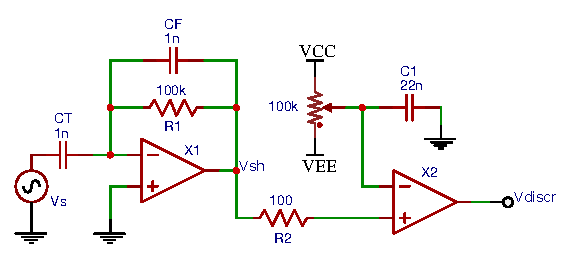
\includegraphics{charge-detector.pdf}
	\caption{Circuito rilevatore di carica.}
	\label{f:circ_detq}
\end{figure}

\begin{table}[h]
	\centering
	\begin{tabular}{S S S S}
		{$C_T$ [\si{\nano\farad}]} & {$C_F$ [\si{\nano\farad}]} & {$R_1$ [\si{\kohm}]} \\
		\midrule
		1.06(7)	&	1.04 (7)	&	98.5(9) \\
	\end{tabular}
	\caption{Valori misurati per i componenti del circuito.}
	\label{t:det_meas}
\end{table}

Si è montato il circuito in \fig{circ_detq}, dove lo scopo del generatore di onde quadre $V_S$, insieme al condensatore $C_T$, è di iniettare nel nostro circuito una carica (che rappresenti ad esempio il segnale di un detector).

Il funzionamento che ci attendiamo, ammettendo l'idealità del generatore, dell'OpAmp e dei condensatori, è il seguente: al fronte di salita (o discesa) di $V_S$ una carica $C_T \Delta V_S $ si deposita sul condensatore $C_F$, portando dunque la tensione $V_{sh}$ a $\frac{C_T}{C_F} \Delta V_S $. La scarica del condensatore attraverso $R_1$ fa sì che la carica su di esso, e quindi la tensione $V_{sh}$, decadano esponenzialmente con un tempo caratteristico $\tau = C_F / R_1$. L'OpAmp $X_2$, configurato come discriminatore con una tensione di soglia positiva (poco inferiore ai \SI{200}{\mV}), ha nel tempo in cui $V_{sh}$ è minore di tale soglia un'uscita $V_{discr}$ negativa ($\approx V_{EE}$); ai fronti di discesa di $V_S$ dunque non ci aspettiamo nessuna variazione dell'output (poichè $V_{sh}$ scende sotto lo 0), mentre ai fronti di salita dovremmo vedere $V_{discr}$ salire a $\approx V_{CC}$ e rimanerci fintantoché $V_{sh}$ non scenda, per lo scaricarsi del condensatore $C_F$, nuovamente al di sotto della tensione di soglia. La \fig{det_norm} riporta i segnali $V_{sh}$ e $V_{discr}$, e si può vedere come le nostre attese siano almeno qualitativamente rispettate.

\begin{figure}[h]
	\begin{subfigure}{0.5 \textwidth}
		\centering
		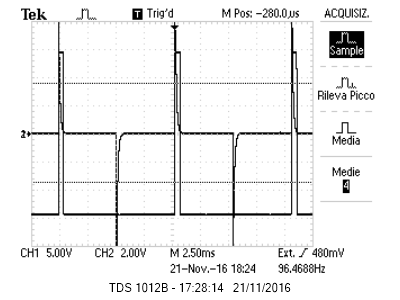
\includegraphics[scale=0.7]{detector.png}
		\caption{Più periodi dell'onda in ingresso.}
	\end{subfigure}
	\begin{subfigure}{0.5 \textwidth}
		\centering
		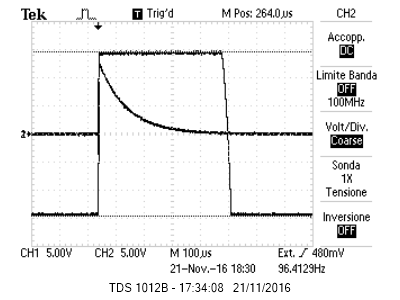
\includegraphics[scale=0.7]{detector_zoom.png}
		\caption{Dettaglio di un singolo evento di rilevazione.}
	\end{subfigure}
	\caption{Andamento di $V_{sh}$ e $V_{discr}$.}
	\label{f:det_norm}
\end{figure}

Si è dunque proceduto a inviare al circuito onde quadre di diversa ampiezza, registrando il corrispondente Time Over Threshold (TOT), ovvero la durata del segnale alto di $V_{discr}$. I dati sono stati usati per un fit del valore della tensione di soglia $V_{th}$ del discriminatore con le caratteristiche date dalle misure in \tab{det_meas}, ottenendo $V_{th} = \SI{0.186 \pm 0.003}{\V}, \ \chi^2 = 3.1 (5 \dof, p=  0.69)$. La possibilità del fit e la compatiblità con quanto atteso mostrano che il circuito è effettivamente ben descritto dal modello sopra esposto; nel grafico in \fig{fit_q} si può notare l'andamento esponenziale della carica depositata nel rilevatore in funzione del TOT.

\begin{figure}[h]
	\centering
	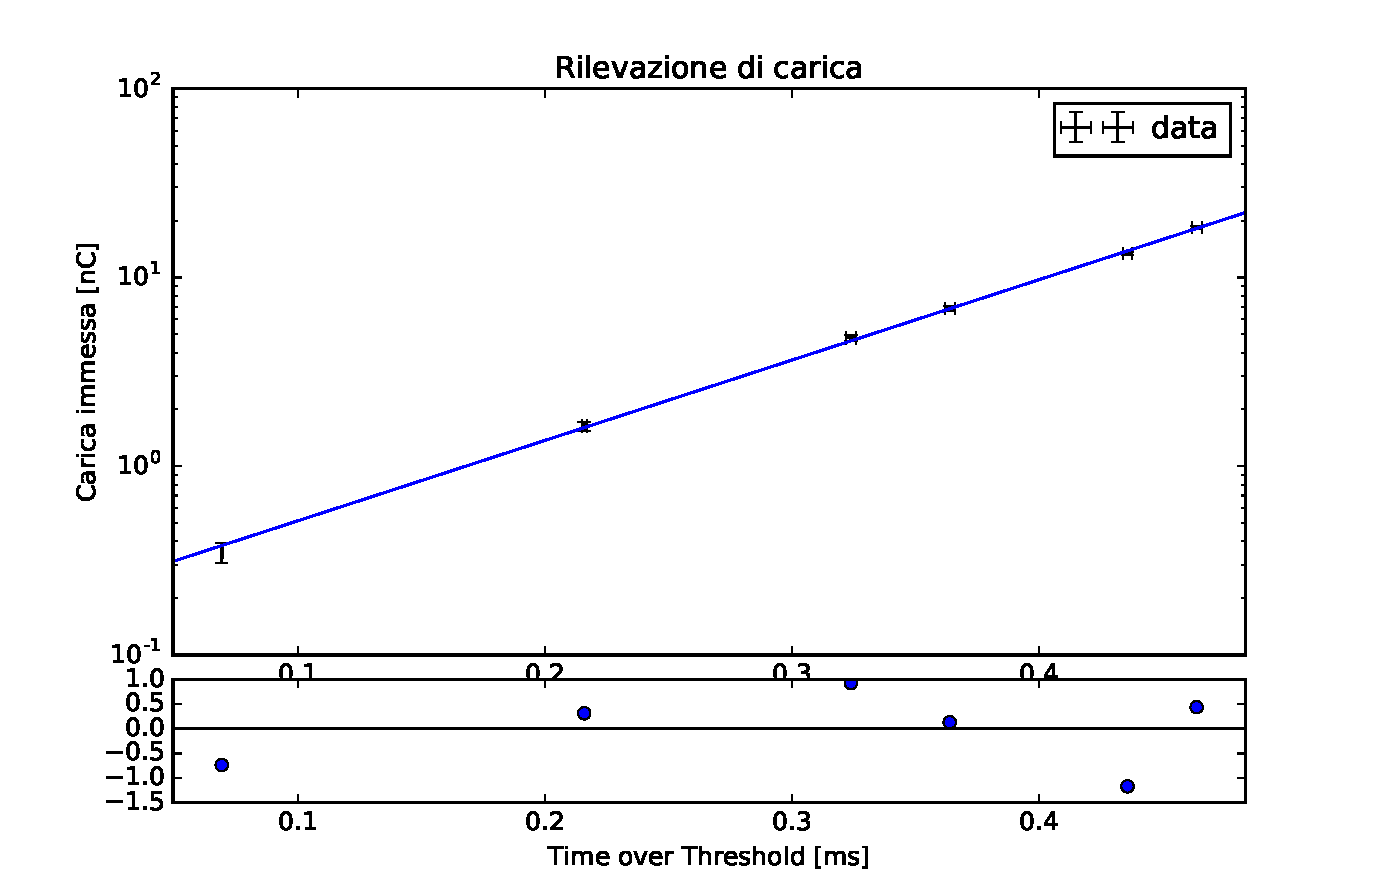
\includegraphics[scale=0.6]{charge_fit.pdf}
	\caption{Fit della carica rilevata in funzione del TOT.}
	\label{f:fit_q}
\end{figure}

Riducendo l'ampiezza dell'onda quadra in ingresso a valori poco maggiori di $V_{th}$, il circuito non dà più una risposta sufficientemente regolare da poterne ricavare informazioni quantitative, come si può vedere in \fig{det_limit}; scendendo ulteriormente al di sotto di $V_{th}$ (o per l'esattezza di $\frac{C_F}{C_T} V_{th}$) in uscita non si osserva puù alcun segnale.
Chiaramente, la tensione di soglia dipende dalla posizione del potenziometro, dunque variandone la regolazione si può tornare a vedere un segnale anche con ampiezza in ingresso più bassa; se invece lo si porta oltre lo 0 (cioè, ad una regolazione tale che la tensione all'ingresso invertente dell'OpAmp $X_2$ sia negativa), si vedrà un output principalmente alto che scende in corrispondenza dei fronti di discesa dell'onda in ingresso (poiché solo in quel momento la tensione $V_{sh}$ può scendere al di sotto della tensione di soglia).

\begin{figure}[h]
	\centering
	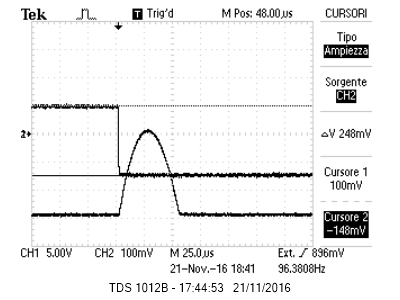
\includegraphics{oltre_limite.png}
	\caption{Andamento di $V_{discr}$ con ingresso di ampiezza troppo ridotta.}
	\label{f:det_limit}
\end{figure}
